\chapter{相位求解：从直接法到似然双空间迭代}
\section{为什么原子性可以提供相位信息}
已知 $|F_h|$ 而未知 $\phi_h$ 时，可以写出许多密度，但绝大多数不会像由少量原子组成的晶体。直接法利用的正是这种结构限制。对足够分离、形状相近的原子峰，密度平方仍在原来的位置有峰，因此 $\rho^2$ 的傅里叶系数与 $\rho$ 的系数近似具有相同相位。傅里叶卷积定理给出
\begin{equation}
 \mathcal F(\rho^2)_h=\frac1V\sum_k F_kF_{h-k},\qquad
 F_h\simeq C_h\sum_kF_kF_{h-k}.
\end{equation}
这是理解 Sayre 方程的出发点\cite{sayre1952}。它依赖原子形状与分离程度；不能把这种近似当成任意无序、缺失反射或任意组成下都成立的精确测量方程。

不同角度的原子散射因子衰减不同。为减少这一影响，可用组成估计一个平均包络，例如
\begin{equation}
 E_h\approx\frac{F_h}{\sqrt{\sum_j f_j^0(s_h)^2}}.
\end{equation}
实际代码还对包络作整体尺度归一化并设置数值下限。这里得到的是用于搜索的归一化振幅，不是重新标定后的实验强度。

\section{三相位不变量与 tangent 更新}
对于 $h=k+l$，令
\begin{equation}
 \Psi_{hkl}=\phi_h-\phi_k-\phi_l.
\end{equation}
移动原点 $o$ 会使 $\phi_h$ 加上 $2\pi h\cdot o$；由于 $h-k-l=0$，$\Psi$ 不变。这解释了直接法为何可以在未知原点的情况下约束相位。

在经典等原子统计近似下，三相位的浓度随 $|E_hE_kE_l|$ 增大，分布可写成 $p(\Psi)\propto\exp(\kappa\cos\Psi)$。把涉及同一 $h$ 的关系相加，最大化余弦一致性，就得到圆周上的加权平均方向\cite{cochran1955,karle1956}：
\begin{equation}
 \phi_h\leftarrow\arg\sum_{k+l=h}w_{hkl}\exp\{\iu(\phi_k+\phi_l)\}.
\end{equation}
0.8.0 构造有预算的稀疏关系图。权重为归一化振幅乘积再乘各观测的可靠性系数；这是一种搜索引导，不声称是复杂组成下精确的相位后验。阻尼更新为
\begin{equation}
 e^{\iu\phi_h^{\rm new}}\ \parallel\
 (1-\lambda)e^{\iu\phi_h}+\lambda
 \frac{\sum_{k+l=h}w_{hkl}e^{\iu(\phi_k+\phi_l)}}{\sum_{k+l=h}w_{hkl}}.
\end{equation}
如果关系之间互相矛盾，圆均值的模会下降，移动也随之减弱。引导强度在后期衰减，最终不要求观测去满足近似的三相位关系。

\section{双空间法与 intrinsic phasing 的位置}
双空间法交替使用两类约束：倒易空间的振幅或相位关系，实空间的原子峰、稀疏性或密度形状。Shake-and-Bake 是这一思路的重要实现\cite{snb1994}。电荷翻转则把低于阈值的密度改变符号，再回到倒易空间更新\cite{charge2004,charge2008}：
\begin{equation}
 D_\delta(\rho)(x)=
 \begin{cases}\rho(x),&\rho(x)\ge\delta,\\-\rho(x),&\rho(x)<\delta.\end{cases}
\end{equation}
这种更新并非普通凸投影，整个过程通常也没有全局收敛保证，因此需要多起点和独立的结构评价。

SHELXT 的 intrinsic phasing 是一个集成体系：Patterson 与双空间过程在 P1 中产生相位，再处理原点、空间群和元素等问题\cite{shelxt2015}。它不是一条可直接替换所有求解问题的单独公式。Ariadne 借鉴这一分解方式，自行实现相位与原点模块；并不包含 SHELXT 的代码或完整内部策略。

Patterson 函数是密度的自相关：
\begin{equation}
 \mathcal P(u)=\frac1V\sum_h|F_h|^2e^{-2\pi\iu h\cdot u}
 =\int_{\text{cell}}\rho(r)\rho(r+u)\,\dif r.
\end{equation}
它的峰反映原子间向量。新求解器以 Patterson 平移后的最小叠合构造部分起点，其余起点为随机密度。这能利用向量信息，又不把原子真值坐标交给求解器。

\section{弱强度需要柔性的倒易更新}
经典振幅替换把当前复数 $v$ 的模强制设为观测振幅。弱反射的 $\sqrt{\max(y,0)}$ 不适合被当成无误差约束。新实现对每个复系数保留当前相位，只求新的模 $r\ge0$：
\begin{equation}\label{eq:prox}
 r^*=\argmin_{r\ge0}
 \left\{\frac{(r-a)^2}{2\tau}+\frac{(r^2-y)^2}{2\sigma^2}\right\},
 \qquad a=|v|.
\end{equation}
第一项限制本次移动，第二项是带符号强度的高斯似然。$\sigma$ 是强度而非振幅的标准不确定度；$\tau$ 是算法参数，不是探测器测量出的方差。

令 $b=\sigma^2/(2\tau)$，驻点方程成为
\begin{equation}\label{eq:cubic}
 r^3+(b-y)r-ba=0.
\end{equation}
当 $a>0$ 时，存在唯一正根：若 $b-y\ge0$，三次式在正半轴严格递增；若 $b-y<0$，它先下降后上升，而在零点的值已经为负，所以也只有一次向上的穿越。$a=0$ 时直接比较边界和驻点，得到 $r^*=\sqrt{\max(y-b,0)}$。

实现使用按尺度归一化的三次方程、双曲函数和 Cardano 分支，避免为每个反射再启动一个优化器。当 $v\ne0$ 时，更新后的复数为 $r^*v/|v|$；当 $v=0$ 时，径向最优值仍由上式确定，但目标函数不区分相位，代码采用 $\arg(0)=0$ 的确定性约定。低不确定度强度约束较紧，高不确定度强度允许模型形状提供更多搜索方向；负 $y$ 同样参与似然。

若强度单位改变为 $y'=cy,\sigma'=c\sigma$，振幅应变成 $r'=\sqrt c\,r$。为保持算法的尺度协变，代码用工作集的归一化正强度均值设定 $\tau$，使 $\tau'=c\tau$。固定一个与单位无关的 $\tau$ 会破坏这一性质。
\begin{figure}[!htbp]
\centering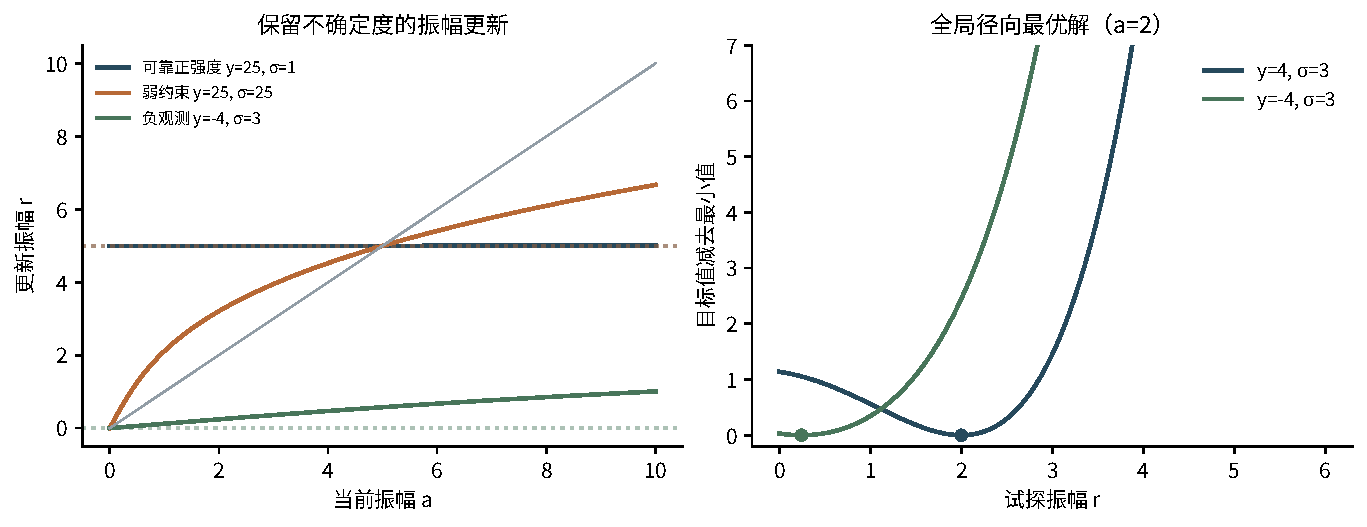
\includegraphics[width=\textwidth]{figures/06_radial_prox.pdf}
\caption{式\eqref{eq:prox}的一维教学示例。横轴是更新前的模，纵轴是求得的模。可靠正强度对目标模约束强；弱正和负强度形成连续、依赖不确定度的更新。虚线是把观测强行转成固定振幅的基线。}
\end{figure}

\section{本版混合求解器的完整循环}
\begin{enumerate}
\item 合并工作集内重复与 Friedel 强度，同时传播方差；验证同一关系轨道没有跨训练和保留角色。实密度求解采用 Friedel 平均，因此不在此步骤推断绝对结构。
\item 按组成建立散射包络、有限三相位图和 FFT 网格。未测到的系数保持为模型变量，不填成“测得的零”。
\item 从随机密度或 Patterson 向量起步；交替作电荷翻转和周期性的有限原子支撑投影。
\item 倒易空间先作衰减的 tangent 引导，再解式\eqref{eq:cubic}。保留 Hermitian 成对关系以及实际倒易度量确定的带宽。
\item 先恢复傅里叶系数的物理散射衰减，再从候选密度提取周期原子峰，用工作强度对候选作初步排序；后续由独立选择集比较精修后的模型。
\end{enumerate}

网格带宽通过倒易度量逐项广播计算，避免同时保存三张完整的整数索引网格。三相位图按候选反射数和每个反射的关系数设上限。多起点仍然是非凸搜索，不能把多跑几轮解释为必定能解。

原有 \code{charge_flip} 与 \code{atomic_projection} 路径保留；新方法名称为 \code{hybrid}。完整晶胞元素数必须由使用者声明。重原子与轻原子混合、分辨率不足、溶剂无序、部分占位和缺失低角反射，都可能削弱原子峰提取。当前实现并未自动推断未知化学式，也未将完全混合的孪晶总强度直接当成一个晶畴的 $|F|^2$。
